\section{Overview of the Hashgraph algorithm}

% insert figure
\tikzset{near start abs/.style={xshift=1cm}}

\begin{figure}
    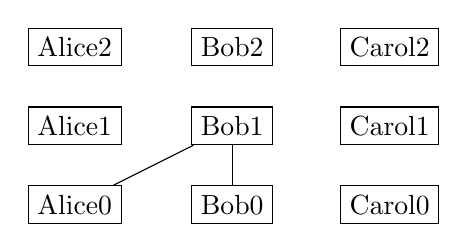
\begin{tikzpicture}
        % place nodes
        \node[draw] at (0, 0)   (a0) {Alice0};
        \node[draw] at (0, 1)   (a1) {Alice1};
        \node[draw] at (0, 2)   (a2) {Alice2};

        \node[draw] at (2, 0)   (b0) {Bob0};
        \node[draw] at (2, 1)   (b1) {Bob1};
        \node[draw] at (2, 2)   (b2) {Bob2};
        
        \node[draw] at (4, 0)   (c0) {Carol0};
        \node[draw] at (4, 1)   (c1) {Carol1};
        \node[draw] at (4, 2)   (c2) {Carol2};

        % draw edges
        \draw[] (a0) -- (b1);
        \draw[] (b0) -- (b1);
        % \draw[] (a) node[above,xshift=1cm] {$x(kT)$} -- (b);
        % \draw[] (c) node[above,xshift=1cm] {$y(kT)$} -- (d);
        % \draw (0,-3) node[above,near start abs] {Test} -- ++(7,0);
    \end{tikzpicture}

    \label{fig:hashgraph}
    \caption{
        Example of how hashgraph spreads information via gossip.
        Alice tells Bob what she knows. 
    }
\end{figure}


Hashgraph uses standard cryptographic hashes and digital signatures to securely spread events across a network by gossipping about gossip(Figure 1).%\ref{fig:hashgraph}).
It was mathematically proven that each member will eventually have a consistent local copy of a Hashgraph for each member to run virtual voting without the need to send votes across the network\cite{baird2016}.

\begin{figure}
    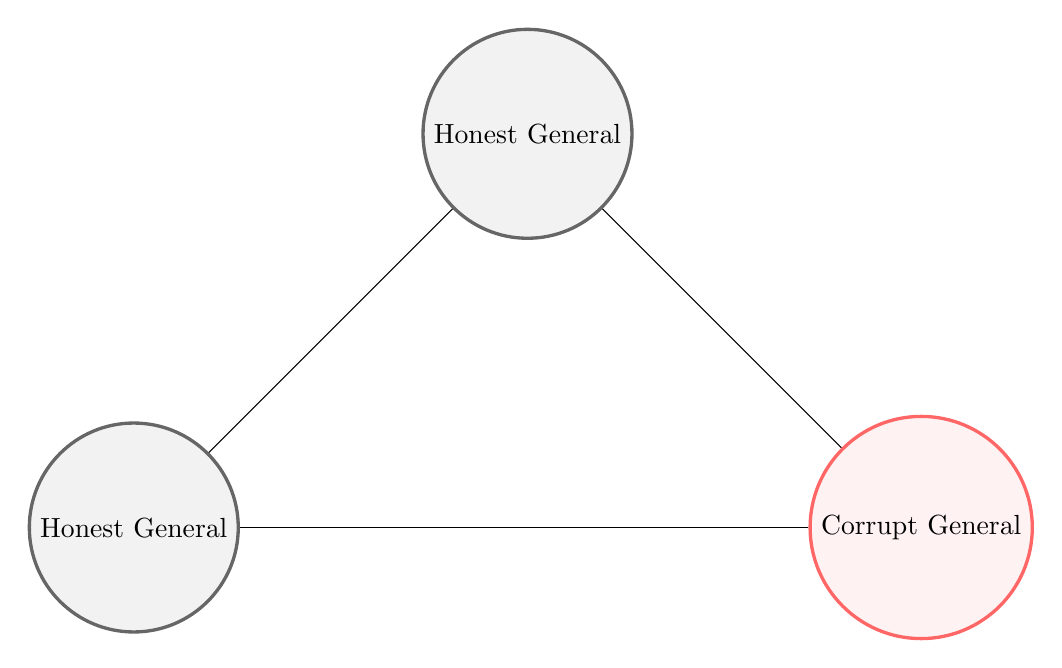
\begin{tikzpicture}[
        roundnode/.style={circle, draw=black!60, fill=black!5, very thick},
        rednode/.style={circle, draw=red!60, fill=red!5, very thick},
        ]

        % Nodes
        \node[roundnode] (a) at (0,0) {Honest General};
        \node[rednode]   (b) at (10,0) {Corrupt General};
        \node[roundnode] (c) at (5,5) {Honest General};
       
        \draw[] (a) -- (b);
        \draw[] (b) -- (c);
        \draw[] (c) -- (a);

    \end{tikzpicture}

    \label{fig:byzantine}
    \caption{
        An illustration of the Byzantine Generals Problem. The Theorem states that consensus cannot be reached if 1/3 or more are malicious.
    }
\end{figure}

% \ref{fig:byzantine}
The Byzantine Generals Problem\cite{shostak1982byzantine} provides the motivation to solve the consensus problem. The theorem illustrated in Figure 2 states that consensus cannot be reliably reached if 1/3 or more are malicious. That is the bound provided by the mathematical theorem in any distributed system. To be Byzantine Fault Tolerant means that a distributed system can withstand failure with some unreliable actors. Asynchronous adds another layer of complexity where messages may get delayed or altered, similar to the real internet with firewalls and denial-of-service attacks. Asynchronous Byzantine Fault Tolerant (aBFT) is the highest level of security a distributed system can achieve\cite{coq2018}.

\begin{figure}
    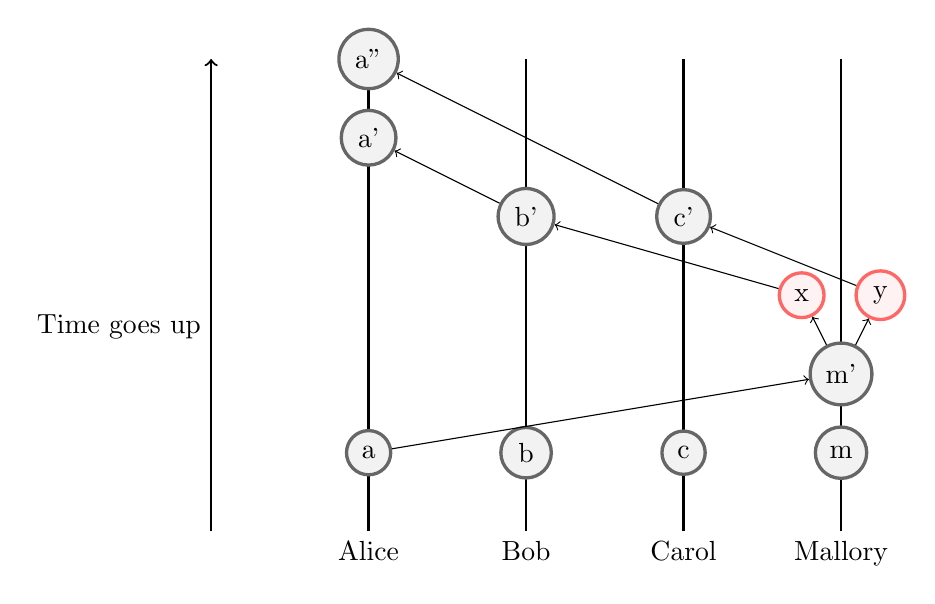
\begin{tikzpicture}[
        roundnode/.style={circle, draw=black!60, fill=black!5, very thick},
        rednode/.style={circle, draw=red!60, fill=red!5, very thick},
        ]
        \draw[thick,->] (0,0) -- (0,2.6) node[anchor=east] {Time goes up} -- (0,6);
        \draw[thick] (2,0) node[anchor=north] {Alice} -- (2,6);
        \draw[thick] (4,0) node[anchor=north] {Bob} -- (4,6);
        \draw[thick] (6,0) node[anchor=north] {Carol} -- (6,6);
        \draw[thick] (8,0) node[anchor=north] {Mallory} -- (8,6);
        
        % Nodes
        \node[roundnode] (a1) at (2,1) {a};
        \node[roundnode] (b1) at (4,1) {b};
        \node[roundnode] (c1) at (6,1) {c};
        
        \node[roundnode] (b4) at (4,4) {b'};
        \node[roundnode] (c4) at (6,4) {c'};

        % Nodes
        \node[roundnode] (m0) at (8,1) {m};
        \node[roundnode] (m1) at (8,2) {m'};
        \node[rednode] (m21) at (7.5, 3) {x};
        \node[rednode] (m22) at (8.5, 3) {y};
      
        % Alice talks to Malory
        \draw[->] (a1) -- (m1);
       
        % Malory cheats
        \draw[->] (m1) -- (m21);
        \draw[->] (m1) -- (m22);

        % Mallory talks to Bob and Carol
        \draw[->] (m21) -- (b4);
        \draw[->] (m22) -- (c4);
       

        \node[roundnode] (a5) at (2,5) {a'};
        \node[roundnode] (a6) at (2,6) {a''};
        \draw[->] (b4) -- (a5);
        \draw[->] (c4) -- (a6);


    \end{tikzpicture}

    \label{fig:cheating}
    \caption{
        Suppose Mallory can cheat by forking an event, eg:
        she could double spend her coins by gossiping two different events (x \& y) to different members. The Strongly Seeing Lemma states that a forked event will not be strongly seen by other members. A proof by contradiction shows that if 2/3 strongly sees x and 2/3 also strongly sees y, then this is impossible to be strongly seen if only less than 1/3 are malicious. If Alice, Bob, and Carol are honest, they will not strongly see Mallory's events as valid.
    }
\end{figure}

% \ref{fig:cheating}
Hashgraph was proven to be aBFT\cite{baird2016}. While a full mathematical proof is beyond the scope of this paper, Figure 3 illustrates it's key pillar of the Strongly Seeing Lemma. Strongly Seeing is one of the key concepts that builds Hashraph's proof that it is aBFT.

In terms of how this translates to its implementation, it is currently a permissioned which relies on no 1/3 or more nodes are malicious. Once it has completed it's path towards decentralisation, it's proof-of-stake system will rely on 1/3 or more of the coins are not owned by malicious actors. 

% \begin{figure}
    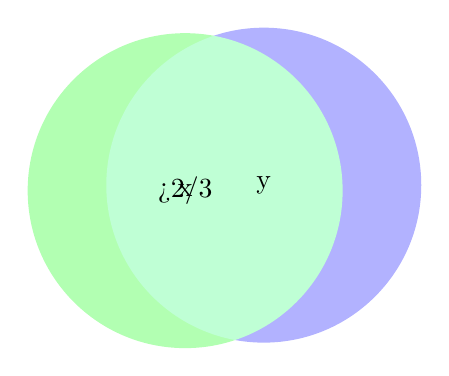
\begin{tikzpicture}
        \begin{scope}[blend group=soft light]
        \fill[green!30!white] (1:2) circle (2);
        \fill[blue!30!white]  (2:3) circle (2);
        \end{scope}

        \node at (1:2)    {x};
        \node at (2:3)    {y};
        \node at (1:2) {>2/3};

    \end{tikzpicture}
    \label{fig:venn}
    \caption{
    }
\end{figure}

% Hashgraph is currently on a path towards decentralisation that will use a proof-of-stake system. 

%As demand rises for a limited supply of coins, it will be extremely difficult for a single actor to.
% To prove how it works, let us define what strongly seeing an event means.

% The Strongly Seeing Theorem <CITE> is the key pillar of how hashgraph works. The proof is by contradiction. Suppose Mallory wants to cheat the system by forking an event. (This is a condensed summary of the proof, see the whitepaper for the full proof) Alice's local hashgraph reads 2n/3 x strongly sees w and another 2n/3 strongly sees y, then the intersection must be >1/3. The assumption is no more than 1/3 is dishonest so there must be an honest member in between. However, that honest member cannot strongly see both events because x and y are fork and breaks the definition of strongly seeing. This is a contradiction therefore the assumption that x strongly sees w is false. Mallory will not be able to cheat if no more than 1/3 of the nodes are malicious.
